\chapter{
Spatial Mark-Resight Models
}

\markboth{Spatial mark-resight models}{}
\label{chapt.partialID}

\vspace{.3in}


So far, we have dealt with the situation where all detected
individuals are
identifiable 
upon encounter because they carry some form of individual mark, and in Chapt. \ref{chapt.scr-unmarked}
we introduced and developed an SCR model for
non-identifiable 
populations, a spatial {\it non}-capture-recapture
model, if you will.
These
two extremes are common in the study of animal populations with
non-invasive sampling methods. However, there is also an intermediate
situation, where 
part of the population is tagged or otherwise
marked and can thus be identified upon recapture, while the unmarked
portion remains unidentified. In this situation so-called mark-resight
models \citep{bartmann_etal:1987, arnason_etal:1991, neal_etal:1993}
can be used to estimate population size and density combining data
from both the marked and unmarked individuals.

Traditionally, 
capture-recapture studies involved physical capture of
individuals throughout the study; 
new individuals are marked on every
re-capture occasion. This methodology is still widely applied in the
study of species that are relatively easy to capture, such as small
mammals, but can be very costly, logistically challenging and risky
when dealing with larger species. In contrast, in mark-resight studies
a sample of individuals is captured and tagged (or otherwise marked)
during a single marking event. Marking is followed by resighting
surveys, upon which both the detection of marked and recognizable
individuals and unmarked animals is recorded. Resighting surveys are
usually non-invasive (hence the name �resighting�), so that they
don't involve handling of animals. As such, mark-resight models have a
major advantage over traditional capture-recapture models in that they
only require individuals to be captured and handled once, during the
initial marking. This reduces field costs and risks for the animals
(and potentially the researchers).

Mark-resight models have a set of underlying assumptions, most of
which are identical
to those of capture-recapture models,
e.g. demographic population closure (violation of geographic
population closure can be accommodated by some models) and no loss or
misidentification of marks (see also Chapt.~\ref{chapt.scr0}).
Just like regular capture-recapture
models, there are means to incorporate heterogeneity in capture
probability. However, a new and essential assumption of mark-resight
models is that the tagged (or otherwise identifiable) individuals are
a representative sample of the study population, so that inference
about detection can be made for the whole population from
the tagged sample. This issue is usually addressed by using a
different method for marking than for resighting, and by marking a
random sample of the population.

Owing to the advantages of mark-resight over capture-recapture,
especially when dealing with hard-to-trap species, mark-resight is a
popular tool in wildlife population studies. The method has been
applied for decades 
to a suite of species and survey techniques,
ranging from banding and resighting Canada geese
\citep{hestbeck_malecki:1989} to ear-tagging and camera-trapping
grizzly bears \citep{mace_etal:1994} to paintball marking and areal
resightings of large ungulates \citep{skalski_etal:2005jwm}.

In this chapter we consider mark-resight in spatial context and
develop a spatial mark-resight (SMR) model. To motivate this model
development, imagine you conduct a live-trapping study during which
you capture and mark a number of animals with individually
recognizable tags. Subsequently, you go back out to the field and
conduct resighting surveys on an array of locations, and during these
resighting surveys you see some of your tagged individuals as well as
new, unmarked ones. Then, for the marked animals you obtain the same
form of spatially explicit individual encounter histories as you would
in a regular SCR study. On top of that you obtain site (and occasion)
specific counts of individuals you did not tag. Thus, spatial
mark-resight is an SCR framework for populations where only part of
the individuals can be identified and the major difference between SCR
and SMR is how we include those counts of unmarked individuals in the
model. In the following sections we first provide some background
information on mark-resight and the types of data such surveys can
provide. We will further explore the implications of the assumption of the marked individuals being a random subset of the population, which, in the context of SMR models refers to both the {\emph demographic composition}, but also to the {\emph spatial distribution of the marked individuals} in {\cal S}. We then move on to the formal development of SMR models,
which, as we will see, are hybrids of regular SCR models and the
models for data without individual identity presented in
Chapt. \ref{chapt.scr-unmarked}. We will look at models for
both known and unknown numbers of marked individuals, and for
imperfect individual identification of marks, and approaches to incorporate telemetry location data. In the spatial
framework, most of the information on model parameters comes from the
marked individuals. But in sec. \ref{partialID.sec.info} we will see
that, analogous to the models we developed in the previous
Chapt. \ref{chapt.scr-unmarked}, the spatial correlation in counts of
unmarked individuals also contributes information about detection and
movement.

\section{Background}
Before we start exploring spatial mark-resight approaches in more detail, we
need to establish some terminology and gain a clear understanding of what types of mark-resight data we can
have, in order to appreciate and understand the different flavors of
mark-resigh models.  

\subsection{Resighting techniques}
As with capture-recapture surveys, there is a range of methods suitable to perform resightings. Common methods are visits to a set of points for resightings by an observer, or camera-trapping; but resightings need not be restricted to a particular set of locations. We can just as well envision a search-encounter kind of method, where a certain area is searched, systematically or oportunistically, for marked animals (see Chapt. \ref{chapt.search-encounter}). In this chapter we will only deal with fixed location resighting surveys, and we will refer to the set of resighting locations as the resighting array. In some instances we will also be concerned with where marked animals were captured, and we refer to these locations as the marking locations. 

\subsection{Types of mark-resighting data}

In general, we have (at least) two sets of data:
encounter histories for marked, and thus,
identifiable 
individuals $i$ at resighting location $j$ and
occasion $k$, $y_{ijk}$, and counts of
unmarked records 
for each
$j$ and $k$, $n_{jk}$.
Depending on the sampling technique, we can
conceive of three slightly different types of partial ID data.


\textbf{(1) Known number of marked individuals:}
If you implement your resighting survey shortly after the marking
session, you may be confident that none of the marked individuals has
died 
or lost its mark. Under these circumstances you know that the
number of marked individuals available for resighting, $m$, is equal
to the number of individuals you tagged. Alternatively, tags might be
radio-transmitters, allowing you to confirm the presence or absence of
marked individuals in the resighting survey area using radio-telemetry
\citep{white_shenk:2001}. In both cases, you know the number of marked
individuals in the population you survey.
In this situation, even though you may fail to resight some of the
tagged individuals, since you know how many there are, you can simply
assign those you never resighted all-zero encounter histories - in other
words, contrary to regular capture-recapture models, in mark-resight
models with a known number of tagged individuals, we can observe
all-zero encounter histories. Under these circumstances, estimating
$N$ reduces to estimating the number of unmarked individuals, $U$.

\textbf{(2) Unknown number of marked individuals:}
If we don't know $m$, for example because we suspect that some of the marks may have been
lost 
between
tagging and conducting the resighting samples, we obtain a slightly
different type of mark-resight data. Here, we do not accurately know the
number of marked individuals available for resighting. As a
consequence, individuals have to be resighted at least once for us to
know they are still tagged and alive and thus available for
resighting. So, contrary to the situation where we know $m$ and
analogous to regular capture-recapture models, we cannot observe
all-zero encounter histories of marked individual. Here, estimating
$N$ involves estimating both $m$ and $U$.

A special case of this kind of data can arise from camera
trapping. Even when dealing with a species that has no spots or
stripes, some individuals in the study population can have natural
marks that make them identifiable on pictures, such as scars or some
distinct coloration. Again, in this scenario an individual has to be
photographed at least once to be known. Here, the fact that both the
``marking'' method and the subsequent resighting method are the same
(although marking in this case does not involve any actual physical
marking) can be cause for concern: our sample of ``marked''
individuals may not be a random sample of the population but consist
of individuals that for some reason are more likely to be
photographed (e.g., individuals with activity center more interior to
the trap array). In that case, a basic assumption of the mark-resight
model is violated.

\textbf{(3) Unknown marked status:}
Finally, consider a scat or hair snare survey, where only a part of
the sample is analyzed genetically (or DNA can only be extracted
from a subset of samples due to sample quality). In this scenario,
your $n_{jk}$ can contain both completely unknown individuals that are
not represented at all in the complete set of encounter histories of marked animals, 
{\bf $Y$}, 
but it can also contain samples
from individuals that we previously identified. The difference is that
in the first two scenarios, part of the population of individuals is
identifiable, while in the second scenario, part of the
sample of individuals is identifiable. This type of data
violates one of the basic assumptions of mark-resight models,
namely, that tagged individuals are always correctly identified as
such.

To our knowledge there are currently no mark-resight models available
that account for possible misidentification of the marking status of
individuals (although some literature is available on
misidentification of individuals in capture-recapture studies, e.g.,
\citealp{yoshizaki_etal:2009, lukacs_burnham:2005,
  link_etal:2010}). In this chapter we will ignore this kind of data
and focus instead on the two types of typical mark-resight data:

\begin{itemize}
\item[(1)] Known number of marked individuals
\item[(2)] Unknown number of marked individuals,
\end{itemize}

For both types of data a slightly different situation arises when in
some instances we can only tell that an individual is tagged, but not
who it is. You may be able to see that an individual is tagged but the
identifying feature of the tag (a number or coloration) may have
become unreadable, or may be hidden from view. In this case, in
addition to data $y_{ijk}$ and $n_{jk}$, you also observe a number of
sightings of marked but unidentified individuals, say $r_{jk}$.

\subsection{A short history of mark-resight models}

Initially, mark-resight methods focused on radio-tagged individuals to
estimate population size \citep{white_shenk:2001}. Radio-collars
provide a means of
determining 
which of the animals are in the study
area and available for sampling, i.e. determining the number of marked
individuals in the population. Knowing this number was a prerequisite
for most earlier mark-resight approaches \citep{white:1996}. The
oldest mark-resight model is the good old Lincoln-Petersen estimator,
 where individuals are marked and a single resight/recapture occasion
 is carried out \citep{krebs:1999}. We need not identify individuals,
 but only tell apart marked from unmarked individuals. Let $m$ be the
 number of marked individuals in the population, $m_{(R)}$ the number
 of marked individuals seen on the resighting occasion, and $n_{(R)}$
 the total number of marked and unmarked individuals observed during
 resighting. Population size $N$ is then estimated as
\[
N = m \times n_{(R)}/m_{(R)}
\]

A suite of more elaborate models using individual capture histories
over several resighting occasions were developed in the 1980s and
90s and compiled into the program NOREMARK \citep{white:1996}. Apart
from the basic model with known number of marked individuals and no
individual variation in resighting probabilities (joint hypergeometric
maximum likelihood estimator) \citep{bartmann_etal:1987,
  white_garrot:1990, neal:1990, neal_etal:1993}, NOREMARK contains
models that account for lack of geographic population closure
\citep{neal_etal:1993}, individual heterogenenity in resighting rates
and sampling with replacement (i.e. individuals can be seen more than
once on any occasion, \citep{minta_mangel:1989, bowden:1993}). A first
mark-resight model allowing for an unknown number of marked
individuals was developed by \citet{arnason_etal:1991}.

While many of these models perform well under certain situations, they
are somewhat
limited in that they
do not allow for combining data across
several surveys \citep{mcclintock_etal:2006} and not all of them are
likelihood-based or allow for different parameterizations (e.g., including a time effect on detection), so that
selection of the most appropriate model cannot be based on standard
approaches such as AIC, but is largely left up to educated guesswork
\citep{mcclintock_etal:2006}. Recently, more flexible and generalized
likelihood-based mark-resight models have been developed. These models
can account for individual heterogeneity in detection, unknown number
of marked individuals and lack of geographical closure, as well as a
less than 100\% individual identification rate of tagged individuals;
they can be applied to sampling with and without replacement and can
combine data across several primary sampling occasions in a robust
design type of analysis
\citep{mcclintock_etal:2009biometrics,mcclintock_etal:2009mdp}. Since
they are all likelihood-based, model selection among different
parameterizations and model averaging based on AIC is an option. Most
of these models have also been incorporated into the program {\bf MARK}
\citep{mcclintock_white:2010}.

For a detailed treatment of these different non-spatial mark-resight
models, we refer you to the original papers cited in the preceding
paragraph. In short, these models are based on the joint likelihood of
two 
model components: one describing the resighting process of
marked individuals (either using a Poisson or a Bernoulli observation
model, depending on whether sampling is with or without replacement),
where resighting probabilities can have both fixed effects to model
individual and environmental covariates, and a random-effect component
to accommodate variation in detection due to individual heterogeneity;
and one describing the number of unmarked individuals observed (or,
under a Poisson observation model, the number of times unmarked
individuals are observed),
$n_t$ ($t$ here and in the following description denotes a primary
sampling occasion, for example, a year or a season; for a
single-season study we could easily drop this subscript) which are
approximated as a normal distribution
\citep{mcclintock_etal:2006}, or a normal distribution left-truncated
at 0 \citep{mcclintock_etal:2009biometrics}:
\[
n_t \sim \mbox{Normal} (\mathbb{E}(n_t), \mbox{Var}(n_t))
\]
Although this is a simplification of the actual sampling process,
\citet{mcclintock_etal:2006} found this normal distribution to be a
satisfactory approximation, which allows $N$ to enter the model
likelihood via $\mathbb{E}(n_t)$ and $\mbox{Var}(n_t)$.

In the simplest model case without any variation in detection, the
expected number of resightings of unmarked individuals,
$\mathbb{E}(n_t)$, can be written as the number of unmarked
individuals times the expected number of detections of a single
individual, which is the mean or expected value of the underlying
observation model:
\begin{equation}
\mathbb{E}(n_t) = (N-m) * \theta
\end{equation}
\label{partialID.eq.E_n}
where $\theta = K \times p$ for a Binomial observation model with $K$
replicates and individual detection probability $p$, or $\theta$ =
expected/average individual encounter rate $\lambda$ for a Poisson
observation model. Similarly, $\mbox{Var}(n_t)$ depends on the
underlying observation model and is based on the parameters that
determine the individual detection probability/encounter
rate. Combining these two components, $N$ is directly incorporated
into the joint likelihood of the model.

While these mark-resight models are very flexible, they
share the shortcomings of traditional capture-recapture models
when it comes to estimating population density (e.g.,
Chapts. \ref{chapt.intro} and \ref{chapt.closed}). As long as
resightings are collected across a number of locations,
however, they come with the same spatial information as (re)captures in
a regular SCR study.
In the following sections we will consider mark-resight sampling in
the framework of spatial capture-recapture. 

\subsection {The random sample assumption}
\label{partialID.sec.random}
In mark-resight studies it is a prerequisite that the marked portion of the studied population is a random sample of that said population, so that detection probability for the population can be adequately estimated from the marked subset. If, for example, there is some latent group structure in your population where one group has a higher detection probability than the other, the marked part of the population should have the same composition with regard to this group structure as the study population. Intuitively, people think of this as a demographic problem. But if you think back to Chapt. \ref{chapt.intro} and one of the motivations for the development of SCR models, this assumption also has spatial implications. In a non-spatial mark-resight study, if all the individuals we mark live on the edge of the resighting array, their exposure to resighting will be lower compared to the exposure of unmarked individuals living in the center of the resighting array, thus artificially deflating estimates of detection. So to obtain a truly random sample of the study population, the {\emph locations of the home ranges} of the marked individuals also have to be a random sample of the home range locations of the entire population. Without a clearly spatially defined population, this is difficult to assess or even to incorporate into study design or analysis.  

In the SMR framework this issue manifests itself more explicitly, for two reasons: (1) we define the spatial context of the population by setting a state-space; and (2) we assume a certain distribution or point process for all individuals within that state-space, in most cases a uniform distribution or homogeneous point process (but see Chapt. \ref{chapt.state-space} for models with inhomogeneous spatial point processes). So, for the marked individuals to be a random subset of the population of {\cal S}, they have to be uniformly disitributed throughout the state-space. When we study a species where some individuals can be identified based on natural marks, while others do not have unique marks (for example regular colored versus melanistic leopards), and we can assume that the distribution of these two groups of individuals across {\cal S} are identical, then the 'random sample' assumption should be met. But what if we actively need to mark individuals in order to distinguish them? It follows that, if we want to meet the random sample assumption, contrary to SCR models, the state-space is no longer a quantity we can set after data collection for analysis purposes, but ideally, we should make definition of  {\cal S} part of our study design. In practical terms, we need to define the state-space, which includes the resighting array plus sufficient buffer to include all animals potentially exposed to this array, and then uniformly mark individual throughout {\cal S}. Alternatively, we could imagine a marking scheme where marking happens uniformly across a larger area or landscape, for example, a large-scale bird banding program, and then resighting happens on a smaller spatial scale within this landscape, so that the state-spacce around the resighting array lies completely within the larger marking area. 

We can see some sampling situations in which either one of the two scenarios might be reasonable, or at least reasonably approximated. For example, later on in this chapter we present a study where raccoons were caught and marked throughout an island, the boundaries of which are a natural limit for the state-space of this particular system. For many studies, however, this might not be the case. Often, marking is the more difficult and logistically challenging part of a mark-resight study -- think about capturing large carnivores. Especially for rare and cryptic species, areas over which resighting is conducted might have to be large to accumulate sufficient data, and marking over an even larger area -- {\cal S} -- would be logistically impossible. So what happens if we capture and mark individuals in a subset of the state-space? Then, while we may well have an overall constant density across {\cal S}, we will have a higher density of marked than unmarked individuals in the vicinity of the marking locations -- live traps, mist nets, whatever is used to catch animals -- and the opposite situation is true as we get further away from the marking locations. You can think about it this way: Animals with activity centers close to marking locations have a higher probability of being caught and marked, so that the closer we are to the marking locations, the higher the proportion of marked individuals relative to unmarked. We have to explicitly take this pattern into account in our model in order to obtain an overall homogeneous distribution of activity centers. As it turns out this is not a trivial problem, but we provide some ideas to approach this problem in later sections of this chapter. For now, we will go on developing SMR models assuming that the marked animals are, indeed, a random sample of the entire population in {\cal S}.


\section{Known number of marked individuals}

We begin with the easiest situation: a known number of
individuals constituting a random, representative sample from the
population are marked and a series of resight samples are conducted
following marking. No marks (or marked animals) are lost between
marking and resighting, all individuals are correctly identified as
marked or unmarked, and marked individuals are 100\% correctly
identified to individual level.

Recall from Chapt. \ref{chapt.scr-unmarked} that without any individual identity, the observed counts at trap
$j$ and occasion $k$, $n_{jk}$, represent the sum of all latent
individual detections at $j$ and $k$,
$\displaystyle\sum\limits_{i=1}^{N} y_{ijk}$, where $y_{ijk}$ are the
latent individual encounter histories.
We can model these counts as
\[
n_{jk} \sim \mbox{Poisson}( \Lambda_{j} )
\]
where
\[
\Lambda_{j} = \sum_{i=1}^{M}( \lambda_{ij} )
\]
Under this formulation, in order to do MCMC,
 we do not need to update the individual
$y_{ijk}$ in our model, which  is more efficient in terms of
computing. However, we can also formulate the model as conditional on
the latent $y_{ijk}$. This is useful because if we have $m$
individually known animals in our study population, than those $m$
$y_{ijk}$ are no longer latent, but fully observed and can easily be
included in the analysis to provide information on detection parameters.

The formulation conditional on $y_{ijk}$ basically brings us back to
the original SCR model, where individual site and occasion specific
counts, $y_{ijk}$, are modeled as
\[
y_{ijk} \sim \mbox{Poisson}(\lambda _{ij})
\]
and
\[
\lambda _{ij} = \lambda_0  \mbox{exp}(-d_{ij}^2/(2 \sigma^2))
\]


Unobserved $y_{ijk}$ are treated as missing data and have to be
updated as part of the MCMC procedure. We can do that by using their
full conditional distribution, which is multinomial with sample size
$n_{jk}$. Let \textbf{u} be an index vector of the $M-m$ hypothetical
unmarked individuals, $u=m+1, m+2, \ldot, M$, and let $\mathbf{y_{ujk}}$ be the vector of observations of {\emph all} individuals in $\mathbf{u}$ at $j$ and $k$. Then 
\[
\mathbf{y_{ujk}} \sim \mbox{Multinomial} (n_{jk}, \mathbf{\lambda_{uj}})
\]

While in the non-spatial mark-resight analysis known individuals
provide direct information about individual detection probability (or
rate), in the spatial setting they also inform
$\sigma$. Including known individuals into the analysis helps estimate
model parameters more accurately and precisely. We will address the
relationship between the number of marked individuals and accuracy of
the estimated parameters in Sec. \ref{partialID.sec.info}.


\subsection{Implementing spatial mark-resight models}
Implementing a spatial mark-resight model in {\bf JAGS} is not
trivial, since the program does not accept partially observed
multivariate nodes (in this case the partially observed individual
encounter histories which we model as coming from a multinomial
distribution). We can, however, work around that by separating the marked from the unmarked data. The {\bf JAGS} code for the model with a known number of marked individuals is shown in Panel \ref{partialID.panel.knownm}. You see that data augmentation is only applied to the unmarked part of the population, and $N$ is the sum of the estimated number of unmarked individuals ({\tt sum(z[])}) and the number of marked individuals, which is known. Also, to reduce run time, we summed observations of marked individuals across occasions and account for that by multiplying $\lambda_{ij}$ with $K$. Although the two data sets are separated, both parts of the population, marked and unmarked, have the same prior uniform distribution of activity centers
A last noteworthy detail in this code is the {\tt dsum()} function. This function is specific to {\bf JAGS} (i.e., you cannot run this model in {\bf BUGS}) and allows you to model data -- here the counts of unmarked individuals, $n_{jk}$ -- as the sum of a number of latent variables -- here the latent erncounter histories of unmarked individuals. While it can be a pain writing out all the arguments of {\tt dsum()}, it is this function that allows us to implement SMR models in {\bf JAGS}.

\begin{panel}[htp]
\centering
\rule[0.15in]{\textwidth}{.03in}
%\begin{minipage}{2.5in}
{\small
\begin{verbatim}
model{

#priors
psi ~ dbeta(1,1)        
lam0 ~ dunif(0, 5)
sigma ~ dunif(0, 5)

#marked part
for(i in 1:m) {
  sm[i,1] ~ dunif(xlim[1], xlim[2])
  sm[i,2] ~ dunif(ylim[1], ylim[2])
  for(j in 1:J) {
    distm[i,j] <- sqrt((sm[i,1]-X[j,1])^2 + (sm[i,2]-X[j,2])^2)
    lambdam[i,j] <- lam0*exp(-distm[i,j]^2/(2*sigma^2))
    y[i,j]~dpois(lambdam[i,j]*K)
    }
  }

##unmarked part
for(i in 1:M) {
  z[i] ~ dbern(psi)
  s[i,1] ~ dunif(xlim[1], xlim[2])
  s[i,2] ~ dunif(ylim[1], ylim[2])
  for(j in 1:J) {
    dist[i,j] <- sqrt((s[i,1]-X[j,1])^2 + (s[i,2]-X[j,2])^2)
    lambda[i,j] <- lam0*exp(-dist[i,j]^2/(2*sigma^2))
    for(k in 1:K) {
      yu[i,j,k] ~ dpois(lambda[i,j]*z[i])
      }
    }
  }

for(j in 1:J) {
  for(k in 1:K) {nU[j,k] ~ dsum(yu[1,j,k],yu[2,j,k],yu[3,j,k],
								[...code shortened...],
								yu[79,j,k],yu[80,j,k])
	}
  }

N <- sum(z[])+m

}
\end{verbatim}
}
%\end{minipage}
\rule[-0.15in]{\textwidth}{.03in}
\caption{
{\bf JAGS} code for SMR model with known number of marked individuals. In this example, $M$, the size of the augmented unmarked data set, is 80. Note that the arguments yu[4,j,k] to yu[78,j,k] of the {\tt dsum()} function are omitted from the code for space reasons.  
}
\label{partialID.panel.knownm}
\end{panel}

Alternatively, we can use the technical skills presented in \ref{chapt.mcmc} XXXX OR CHANGE TO APPENDIX XXX and derive our own MCMC algorithm. To do so, we only have to make relatively
simple modifications to the MCMC code we developed for regular SCR models in
Chapt. \ref{chapt.mcmc}.
Essentially, since we observe individual detections for the marked part of the population, we have to update only the unobserved part of the full -- augmented -- set of encounter histories, ${\bf Y}$, and
modify the updating steps for $z_i$ and $\psi$, the parameters introduced by data augmentation, to reflect that these only apply to the unmarked part of the population, in other words, to the $M-m$ individuals in our data. You can find the full MCMC code in the accompanying {\bf R} package {\tt scrbook} by invoking {\tt scrPID}. The R code below shows how to simulate SMR data using the {\tt scrbook} function {\tt sim.pID.data}, and running an SMR model on the data, both in {\bf JAGS} and using {\tt scrPID}. The model file {\tt mknown.jag} in the {\tt jags.model} call should contain the code from Panel \ref{partialID.panel.knownm}.

{\small
\begin{verbatim}
set.seed(2013)
N=80 # pop. size
m<-45 # no. marked
sigma=0.5
lam0=0.5
K=5
#make resighting array
gx<-gy<-seq(0,6,1)
X<-as.matrix(expand.grid(gx, gy))
J=dim(X)[1]
#limits of S
xlims<-ylims<-c(-1.5, 7.5)
#simulate data
dat=sim.pID.data(N=N, K=K, sigma=sigma, lam0=lam0, knownID=m, X=X, xlims=xlims, 
				ylims=ylims, obsmod='pois',	nmarked='known')

### prep data for analysis in JAGS
n<-dat$n-apply(dat$Yknown,2:3,sum)
y<-apply(dat$Yknown,1:2,sum)

M<-80 #augmentation only for unmarked

#initial values for latent y
yin<-array(0, c(M,J,K))
for(j in 1:J){
for(k in 1:K){
yin[1:M,j,k]<-rmultinom(1, n[j,k], rep(1/M, M))
}}

data<-list(y=y, nU=n, m=m, M=M, J=J, X=X, xlim=xlims, ylim=ylims, K=K)
inits<-function(){list(sigma=runif(1), lam0=runif(1), 
			sm=cbind(runif(m, xlims[1], xlims[2]), runif(m, ylims[1], ylims[2])),
			s=cbind(runif(M, xlims[1], xlims[2]), runif(M, ylims[1], ylims[2])),
			z=rep(1, M),yu=yin)}
params<-c('lam0', 'sigma', 'N', 'psi')

#analysis in JAGS
library(rjags)
mod<-jags.model('mknown.jag',data, inits, n.chains=1, n.adapt=800)
out<-coda.samples(mod,params, n.iter=5000)

#analysis with scrbook MCMC code
library(scrbook)
library(coda)
inits2<-function(){list(psi=runif(1), sigma=0.5, lam0=0.5, 
		S=cbind(runif(M+m, xlims[1],xlims[2] ), runif(M+m, ylims[1],ylims[2])))}
out2<-scrPID(n=n, X=X, y=dat$Yknown, M=M+m, obsmod = "pois", niters=5800, 
		xlims=xlims, ylims=ylims,inits=inits2(),delta=c(0.1,0.1,0.5))
\end{verbatim}
}
You can look at the two sets of output invoking {\tt summary(out)} for the {\bf JAGS} analysis and {\tt summary(window(mcmc(out2),start=801))} for the custom MCMC algorithm, excluding the first 800 iterations (analogous to the adaptive phase in {\bf JAGS}). We summarized the results in Table \ref{partialID.tab.knownm}. We see that there is some positive bias in estimates of $N$, but credible intervals overlap the true value (80). As expected, estimates from both implementations are very similar; slight differences are probably the result of the relatively low number of iterations.  
You will find that sometimes, {\bf JAGS} produces an error message, upon trying to compile the model, saying that some of the observed $y$ are inconsistent with parent nodes at initialization. We have mentioned before that  {\bf JAGS} is very sensitive to initial values and we believe this is what is happening here. If this error occurs, just repeat the {\tt jags.model} command, usually, model compilation is successful on a second attempt (assuming, of course, that you followed the code above correctly). We further find that the custom MCMC alorithm tends to be faster than {\bf JAGS}, which is why the examples and simulation studies shown in the following sections were run solely in {\bf R}.

\begin{table}
\label{partialID.tab.knownm}
\centering
  \caption{Posterior summaries of the spatial mark-resight model with known number of marks, analyzed in JAGS and using {\tt scrPID}.}
  \begin{tabular}{lcccccc}
             \hline
  Implementation & Parameter &   Mean &   SD &  2.5\% & 50\% & 97.5\% \\
           \hline
{\bf JAGS} & $N$      & 88.72 & 6.75 & 77 & 88 & 103 \\
			& $\lambda_0$  &  0.53 & 0.08 & 0.39 & 0.53 & 70 \\
			& $\sigma$ &  1.29 & 0.02 & 1.26 & 1.30 & 1.32 \\
			& $\psi$    & 0.47   & 0.03  & 0.45  & 0.47 & 0.53  \\
		\hline
{\tt scrPID}& $N$      & 86.01 & 7.58 & 73 & 85 & 102 \\
			& $\lambda_0$  &  0.54 & 0.08 & 0.39 & 0.53 & 0.72 \\
			& $\sigma$ &  0.48 & 0.03 & 0.42 & 0.48 & 0.53 \\
			& $\psi$    & 0.51   & 0.11  & 0.32  & 0.51 & 0.73 \\
			\hline
  \end{tabular}
\end{table}


\section {Unknown number of marked individuals}
\label{partialID.sec.unknown}
Now let us consider the case where we do not know the exact number of
tagged individuals available for resighting so that we have to capture
an individual at least once to be sure that it is available. Unless we
have a direct means of confirming the number of marked animals
available for resighting, treating this number as unknown is probably
more realistic
 in most circumstances. As a consequence of not knowing the exact number of marked individuals, we cannot observe all-zero encounter histories. When using maximum likelihood inference, this situation requires a model where detection rates of known individuals are modeled using a zero-truncated distribution \citep{mcclintock_etal:2009biometrics}. If we did not account for the fact that zeros are unobservable, our estimates of detection rates would be artificially inflated and estimates of population size would be negatively biased.

Working with zero-truncated distributions in a spatial mark-resight
setting is less straight-forward than for non-spatial mark-resight. A
marked individual only has to show up once, anywhere on the resighting
array,
for us to know that it is there. When resightings are pooled
across the entire sampling grid, then the total individual counts $\sum_j y_{ijk}$ have to be $>$ 0 for all resighted individuals and a zero-truncated distribution can be used to model these counts. However, we are concerned with trap-specific encounters, $y_{ijk}$, which can easily be 0 for a resighted individual, as long as a single $y_{ij}$ is $>$ 0. Thus, the zero-truncation does not apply to the individual and trap specific counts we observe, but only to the sum of these counts over all traps.

As an alternative to a zero-truncated distribution, in a Bayesian
framework, we can make use of data augmentation to estimate the number
of marked individuals \citep[e.g.,]{mcclintock_hoeting:2010}. In the SMR framework that means that we create two augmented data sets, one for the marked individuals and one for the unmarked, and estimate their number separately, having them share the parameters of the detection model. Sometimes we may know the maximum number that were ever marked before a resighting survey, in which case we can use that number as the data augmentation limit for the marked data set. Panel \ref{partialID.panel.unknownm} shows the {\bf JAGS} code for the SMR model with unknown number of marks, which is identical to the one in Panel \ref{partialID.panel.knownm}, but for the augmentation of the marked data set. This introduces both a data augmentation parameter, {\tt psim}, and an auxiliary ``alive state'' variable, {\tt zm[i]}, into the description of the marked data model. Again, we provide an alternative, {\bf R}-only MCMC algorithm within {\tt scrbook} -- {\tt scrPID.um}. 

\begin{panel}[htp]
\centering
\rule[0.15in]{\textwidth}{.03in}
%\begin{minipage}{2.5in}
{\small
\begin{verbatim}
model{

#priors
psim ~ dbeta(1,1) 
psi ~ dbeta(1,1)        
lam0 ~ dunif(0, 5)
sigma ~ dunif(0, 5)

#marked part
for(i in 1:max) {
  zm[i]~dbern(psim)
  sm[i,1] ~ dunif(xlim[1], xlim[2])
  sm[i,2] ~ dunif(ylim[1], ylim[2])
  for(j in 1:J) {
    distm[i,j] <- sqrt((sm[i,1]-X[j,1])^2 + (sm[i,2]-X[j,2])^2)
    lambdam[i,j] <- lam0*exp(-distm[i,j]^2/(2*sigma^2))*zm[i]
    y[i,j]~dpois(lambdam[i,j]*K*zm[i])
    }
  }

##unmarked part
for(i in 1:M) {
  z[i] ~ dbern(psi)
  s[i,1] ~ dunif(xlim[1], xlim[2])
  s[i,2] ~ dunif(ylim[1], ylim[2])
  for(j in 1:J) {
    dist[i,j] <- sqrt((s[i,1]-X[j,1])^2 + (s[i,2]-X[j,2])^2)
    lambda[i,j] <- lam0*exp(-dist[i,j]^2/(2*sigma^2))
    for(k in 1:K) {
      yu[i,j,k] ~ dpois(lambda[i,j]*z[i])
      }
    }
  }

for(j in 1:J) {
  for(k in 1:K) {nU[j,k] ~ dsum(yu[1,j,k],yu[2,j,k],yu[3,j,k],
								[...code shortened...],
								yu[79,j,k],yu[80,j,k])
	}
  }

Nu <- sum(z[])
Nm<-sum(zm[])
N<-Nu+Nm

}
\end{verbatim}
}
%\end{minipage}
\rule[-0.15in]{\textwidth}{.03in}
\caption{
JAGS code for SMR model with unknown number of marked individuals. In this example, $M$, the size of the augmented unmarked data set, is 80. Note that the arguments yu[4,j,k] to yu[78,j,k] of the {\tt dsum()} function are omitted from the code for space reasons.  
}
\label{partialID.panel.unknownm}
\end{panel}

Note that we could look at the problem of not knowing the number of marked individuals in the study population as a manifestation of a lack of population closure. In other words, marked individuals may have emigrated, died or lost their marks in the time between marking and resighting. If we have information on the rates of these events, or a series of resighting surveys, we could develop an open population model for the marks in our population and estimate their number at a given resighting survey in this fashion. This kind of SMR model remains to be explored. 

\subsection{Canada geese in North Carolina}

We applied the spatial mark-resight model with an unknown number of
marks and a binomial encounter process to a dataset of Canada goose
resightings \citep{rutledge:2012} XXXget full citation with
LizXXX. During the molt of 2008, 751 individual geese were captured
and marked with neck and leg bands in Greensboro, North Carolina
(Fig. \ref{partialID.fig.geese}). Geese were resighted at 87 
locations 
on 81 resighting events over a period of 18 months. In addition to the
banded geese, the number of unmarked geese was recorded during each
resighting event. Here, we only looked at a subset of the data, from
mid July to the end of October 2008, which corresponds to the first
part of the post-molt season, before migratory Canada geese arrive in
North Carolina. We treated this population as closed over this period. 
During this part of the study, 57 of the resighting sites vere visited and $n = 654$ marked geese were resighted 3994 times at 40 different sites. In addition, 7944 sightings of unmarked geese were recorded at 48 sites.

In the model, we allowed $\sigma$ to vary between males and
females. We set the size of the augmented unmarked data set to 7000. We used the total number marked geese (751) as the upper limit for the augmented marked data set. We ran 50000 MCMC iterations and removed a burn-in of 5000 iterations. To describe the state-space, we buffered the resighting locations by 4.5 km. We assumed that marked geese were a random sample from the state-space, which seems reasonable because (a) marking took place across most of the extent of the resighting array; and (b) marking was done during the molting period, when geese are fairly immobile, and it seems resonable to assume that, once the molt is complete, the marked geese redistributed themselves. We provide all the data ({\tt data(`geesedata')}) and functions ({\tt geeseSMR}) for you to repeat this analysis but be aware that given the large data set it will take days to do so. The {\bf R} code to set up the data and run 5000 iterations of the goose model is given as an example on the help page for {\tt geeseSMR}. The model results, including the derived parameter density ($D$) in individuals per $km^2$ are shown in Tab. \ref{partialID.tab.geese}.


\begin{table}
\label{partialID.tab.geese}
\centering
  \caption{Posterior summaries of the spatial mark-resight model for Canada geese in North Carolina. $N$ is the total population size of marked and unmarked individuals; $m$ is the number of marked individuals.}
  \begin{tabular}{lccccc}
             \hline
       &   Mean &   SD &  2.5\% & 50\% & 97.5\% \\
           \hline
$m$      &  739.77 & 3.24  &  733 & 740  & 746 \\
$N$      & 5756.10 & 90.68 & 5577 & 5757 & 5932 \\
$D$       &  13.76 & 0.19 & 13.38 & 13.76 & 14.14 \\
$\lambda_0$ &  0.19 & $<$0.01 & 0.18 & 0.19 & 0.19 \\
$\sigma$, females  &  1.29 & 0.02 & 1.26 & 1.30 & 1.32 \\
$\sigma$, males  &  1.06 & 0.02 & 1.02 & 1.06 & 1.11 \\
$\psi$, marked    & 0.99 & $<$0.01 & 0.98  & 0.99  & 0.99 \\
$\psi$, unmarked   & 0.72  & 0.01 & 0.69 & 0.72  & 0.74 \\
$\phi$     &  0.36 & 0.02 & 0.32 & 0.36 & 0.39 \\
    \hline
  \end{tabular}
\end{table}

We see that credible intervals of estimates are pretty narrow, surely an effect of the large data set. Estimates of $m$ indicate that most of the 751 geese originally banded are still alive and marked, which is not surprising, given that not much time passed between marking and this first resighting session. The parameter $\phi$ in this model is the probability of being a male, a measure of the sex ratio of the population, which is slightly biased in favor of females.

\begin{figure}[ht]
  \centering
  \includegraphics[width=3in]{Ch19-PartialID/figs/Geese_pic2.png}
  \caption{Banded and unbanded Canada geese in a parking lot in Greensboro, North Carolina.
({\it Photo credit: M.E. Rutledge, NCSU Canada goose project})}
  \label{partialID.fig.geese}
\end{figure}


\section  {Imperfect identification of marked individuals}
\label{partialID.sec.IDrate}

Often during resighting, it may be possible to see that an individual
is tagged but impossible to determine its individual identity. In such
a situation in addition to the $y_{ijk}$ and $n_{jk}$, we also have
site and occasion specific counts of marked but unidentified
individuals, $r_{jk}$. Here, the individual encounter histories of
marked animals are incomplete, and if we used these incomplete data to
inform the detection parameter of the model, we would run the risk of
underestimating detection/trap encounter rate and overestimating
abundance. Some non-spatial mark-resigh models do not require that
marked animals be identified individually, as long as the marking
status can be observed unambiguously, but ignoring individual level
information means that we cannot accommodate heterogeneity in
detection \citep{mcclintock_white:2010}. In a spatial framework we
could ignore marked and unmarked status completely and apply the model
by \citet{chandler_royle:2012} we discussed in
Chapt. \ref{chapt.scr-unmarked}. But, that would mean losing
important information on individual detection and movement. Therefore,
being able to retain the individual identity of records that can be
identified while at the same time accounting for imperfect identification of marked individuals is extremely useful.

\citet{mcclintock_etal:2009biometrics,mcclintock_etal:2009mdp} suggest
an intuitive means of correcting for this bias in a non-spatial model
framework when dealing with a Poisson encounter model (or sampling
with replacement). When marked but unknown resightings are part of the
data, the expected number of records of unmarked individuals, $n$, changes from Eq. \ref{partialID.eq.E_n} to:
\[
E(n) = (N-m) { \lambda  + \eta/m}
\]
Here, $\lambda$ is the individual encounter rate estimated from the known resighted individuals and $\eta$ is the number of records of marked but unidentified individuals. So, because the observed $\lambda$ is known to be too low, the average number of unidentified pictures per known individual is added as a correction factor. This procedure assumes that the inability to identify a marked individual occurs at random throughout the population, which seems to be a reasonable assumption under most circumstances.


We can 
translate this concept to our spatial
mark-resight models. In the spatial model framework we are interested
in the individual and trap specific encounter rate,
$\lambda_{ij}$. Further, we do not look at the sum of all records of
unmarked individuals, but formulate the model conditional on the
latent individual encounter histories. Thus, instead of using $\eta/m$
as a correction factor, we need something that applies at the
individual and trap level. If we take the sum of all correctly
identified records of marked individuals, $\sum y_c$ and divide it by
the total number of records of marked individuals, $\sum y_m$, we get
the average rate of correct individual identification for marked
individuals, say, $c$:
\[
c = \sum y_c/\sum y_m
\]
We could then apply $c$ as a correction factor for $\lambda_0$ for the marked individuals.

A more formal, model-based way to specify $c$ is by assuming that
\[
\sum y_c \sim \mbox{Binomial}(\sum y_m, c)
\]
and estimating $c$ as another model parameter, so that we account for the uncertainty about it. 
For the marked individuals we can then multiply $\lambda_0$
by $c$ to account for the fact that we observe incomplete individual
encounter histories. Since we don't have this identification issue for
unmarked individuals, their baseline trap encounter rate remains as
before simply $\lambda_0$ (or in other words, $c$ for unmarked individuals equals 1). 

Incomplete individual identification of marked
individuals is easily incorporated into our {\bf JAGS} model, no matter whether $m$ known or unknown, by adding the following two lines of code:
{\small
\begin{verbatim}
c~dbeta(1,1) #prior for c
npics[1]~dbin(c, npics[2]) #model for c
\end{verbatim}
}
and modifying the marked observation model description to
{\small
\begin{verbatim}
y[i,j]~dpois(lambdam[i,j]*c*K)
\end{verbatim}
}
It is also included as an option in the {\tt scrPID} and  {\tt scrPID.um} functions. Choosing an uninformative (and conjugate) $\mbox{beta}(1,1)$ prior for $c$, within the {\tt scrPID} algorithm we can update $c$ directly from its full conditional distribution, which is $\mbox{beta}(1 + \sum y_c, 1 + (\sum y_m-\sum y_c))$.
We show an example of using $c$ in an analysis in
sec. \ref{partialID.sec.telemetry}.

Observe that now, in addition to assuming that failure to identify
tagged individuals occurs at random throughout the population, we also
assume that it occurs at random throughout space, i.e. our success of
identifying a tagged individual does not depend on the trap we
encounter it in. As long as individuals are identified based on the same type of tags
the assumption that failure to identify marked individuals occurs at
random throughout the population should be valid. The assumption that
failure to identify marked individuals occurs at random in space could
be violated, for example when spatially varying habitat conditions
influence the ability to recognize individual tags, or when an
observer effect influences individual identification rates. While we
haven't experimented with it, we believe that the approach
described above could readily be extended to account for these
differences. For example, identification rates could be calculated
separately for different observers, or be modeled as functions of
habitat covariates. As an alternative to the approach we present here,
model development could explore assigning records of marked but
unidentified individuals to marked individuals in a fashion similar to
how unmarked records are assigned to hypothetical individuals in this
model, namely, based on the location of the record and the estimates
of home range centers of marked individuals. While this is
computationally more advanced it would make full use of the spatial
information of the unmarked records.



\section{How much information do marked and unmarked individuals contribute?}
\label{partialID.sec.info}
It is intuitive that having marked individuals in the study population should lead to more accurate and precise parameter estimates than when no individuals are identifiable. To evaluate how strongly adding marked individuals to a population improves parameter estimates, \citet{chandler_royle:2012} performed a simulation study. They used a 15 $\times$ 15 resighting grid and
simulated detection data of $N = 75$ individuals in a 20 $\times$ 20 units state-space over $k = 5$ occasions with
$\sigma = 0.5$ and $\lambda_0 = 0.5$. They generated 100 datasets each for
$m$ = (0, 5, 15, 25, 35) where $m$ is the known number of marked individuals randomly sampled from the population.

\begin{figure}[ht]
  \centering
  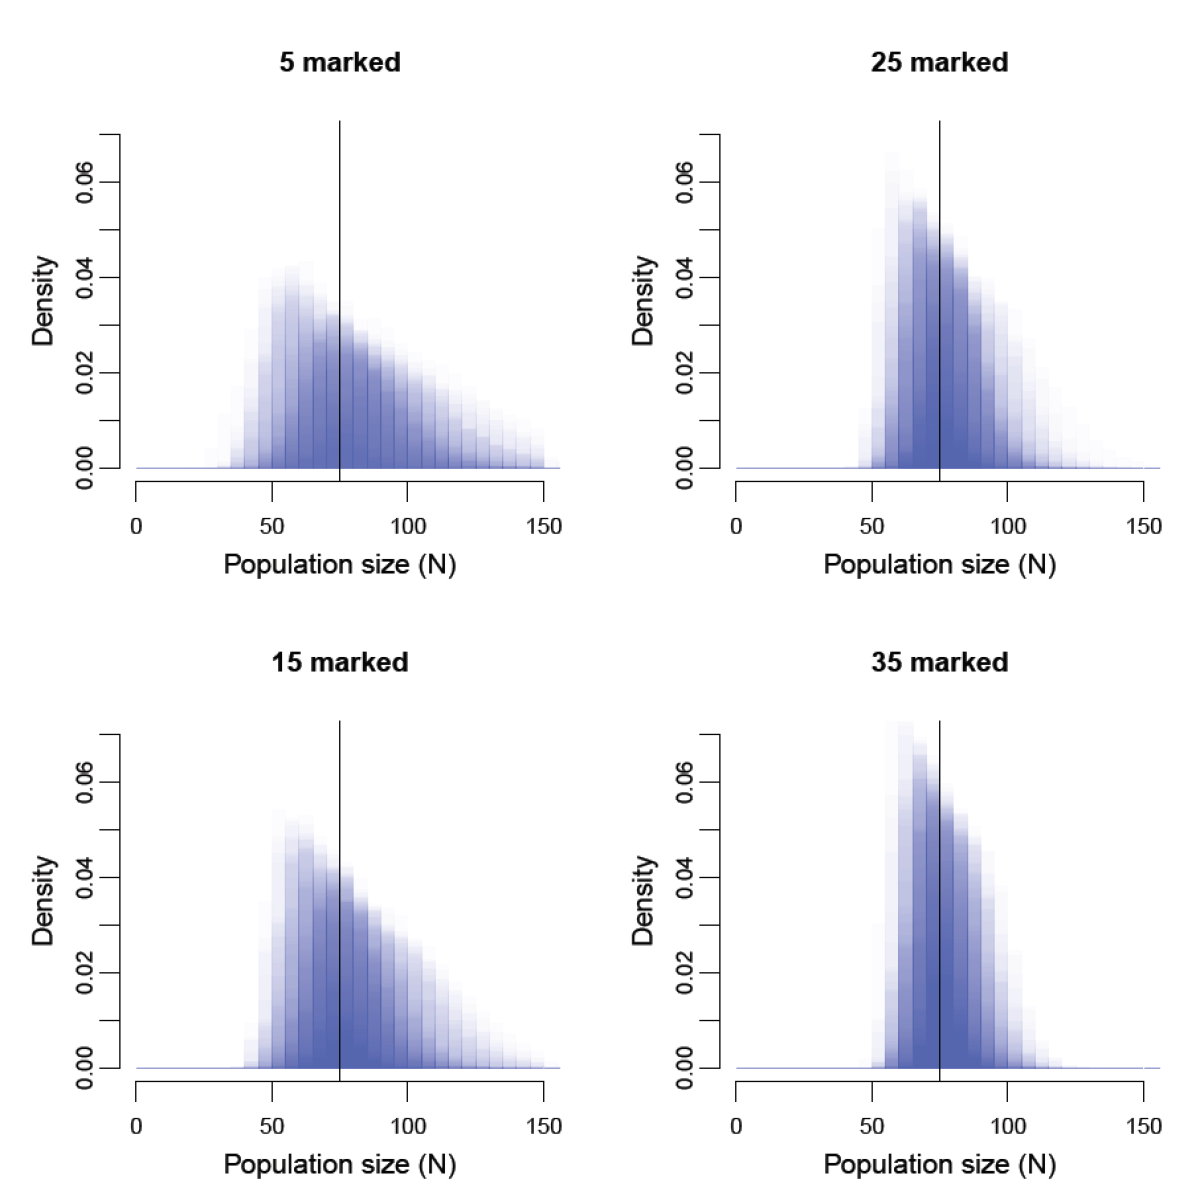
\includegraphics[width=4in,height=4in]{Ch19-PartialID/figs/Nposts2.png}
  \caption{Overlaid posterior distributions of $N$ from 100 simulations
    for four levels of marked individuals.}
  \label{partialID.fig.nposts}
\end{figure}

Without any marked individuals in the population, the posterior
distribution of $N$ turned out to be highly skewed, but its mode was
still an approximately (frequentist) unbiased point estimator of
$N$. As anticipated, posterior precision increased substantially with
the proportion of marked individuals (Tab. \ref{partialID.tab.sim} and
Fig. \ref{partialID.fig.nposts}). The posterior mode was approximately
unbiased as a point estimator, and the relative root-mean squared
error decreased from 0.246 when no individuals were marked to 0.085
when 35 individuals were marked
(Tab. \ref{partialID.tab.sim}). Coverage was nominal for all values of
$m$ and posterior skew greatly diminished with increasing $m$ (Tab. \ref{partialID.tab.sim}).


\begin{table}[ht]
\centering
\caption{Posterior mean, mode, and associated relative RMSE for simulations in
  which $m$ of $N$=75 individuals were marked. One hundred simulations of each case were conducted. }
\begin{tabular}{llrrrrr}
     \hline
     &	Parameter    &	Mean   &	rRMSE  & Mode   & rRMSE &	BCI    \\
     \hline
 m=0 &	$N$          &	85.866 &    0.259 & 77.720 &    0.242 & 0.950  \\
     &	$\lambda_0$  &	0.506  &	0.180 &	0.488  &	0.182 &	0.960  \\
     &	$\sigma$     &	0.495  &	0.115 &	0.486  &	0.113 &	0.960  \\
     \hline
 m=5 &	$N$          &	80.898 &    0.184 & 76.360 &    0.182 & 0.970  \\
     &	$\lambda_0$  &	0.510  &    0.178 & 0.494  &    0.180 & 0.950  \\
     &	$\sigma$     &	0.496  &    0.089 & 0.488  &    0.086 & 0.970  \\
     \hline
 m=15&	$N$          &	79.028 &    0.148 & 76.250 &    0.147 & 0.950  \\
     &	$\lambda_0$  &	0.508  &    0.163 & 0.494  &    0.164 & 0.950  \\
     &	$\sigma$     &	0.496  &    0.073 & 0.492  &    0.071 & 0.970  \\
     \hline
 m=25&	$N$          &	77.765 &    0.114 & 75.810 &    0.113 & 0.950  \\
     &	$\lambda_0$  &	0.511  &    0.153 & 0.498  &    0.157 & 0.950  \\
     &	$\sigma$     &	0.496  &    0.067 & 0.493  &    0.065 & 0.940  \\
     \hline
 m=35&	$N$          &	76.446 &    0.085 & 74.900 &    0.085 & 1.000  \\
     &	$\lambda_0$  &	0.513  &    0.142 & 0.501  &    0.144 & 0.950  \\
     &	$\sigma$     &	0.497  &    0.056 & 0.493  &    0.057 & 0.940  \\
 \hline
\end{tabular}
\label{partialID.tab.sim}
\end{table}

As we saw in the previous chapter, the spatial correlation in unmarked counts can be sufficient to obtain estimates of movement and detection parameters. However, only marked and thus identifiable individuals provide us with direct information about these parameters and may well dominate estimates.
To single out the contribution of marked and unmarked individuals to parameter estimates, we re-ran the same simulations but let $\sigma$ and $\lambda_0$ be updated based solely on the data of marked individuals. Results are summarized in Tab. \ref{partialID.tab.sim2}.
We see that if we update $\lambda_0$ and $\sigma$ based on marked individuals only, estimates of these parameters are more biased and less precise. For estimates of $N$, especially for $m$= 5 and $m$ = 15, we observe a stronger positive bias, lower accuracy and considerably lower BCI coverage as compared to when both marked and unmarked individuals contribute to parameter estimates (Tab. \ref{partialID.tab.sim2}). Thus, unmarked individuals do actually contribute noticeably to estimating model parameters.

\begin{table}[ht]
\centering
\caption{Posterior mean, mode, and associated relative RMSE for simulations in
  which $m$ of $N$=75 individuals were marked and unmarked individuals
  did not contribute to estimating $\lambda_0$ and $\sigma$.
  One hundred simulations of each case were conducted. }
\begin{tabular}{llrrrrr}
\hline
     &	Parameter    &	Mean   &	RMSE  &	Mode   &	RMSE &	BCI    \\
     \hline
 m=5 &	$N$          &	88.621 &	0.369 &	83.139 &	0.421 &	0.810  \\
     &	$\lambda_0$  &	1.255  &	1.247 &	0.606  &	1.148 &	0.950  \\
     &	$\sigma$     &	0.472  &	0.252 &	0.426  &	0.333 &	0.910  \\
     \hline
 m=15&	$N$          &	81.031 &	0.192 &	78.361 &	0.175 &	0.820  \\
     &	$\lambda_0$  &	0.535  &	0.281 &	0.476  &	0.284 &	0.970  \\
     &	$\sigma$     &	0.503  &	0.109 &	0.490  &	0.107 &	0.940  \\
     \hline
 m=25&	$N$          &	78.206 &	0.129 &	76.594 &	0.123 &	0.920  \\
     &	$\lambda_0$  &	0.531  &	0.204 &	0.496  &	0.202 &	0.960  \\
     &	$\sigma$     &	0.497  &	0.081 &	0.489  &	0.084 &	0.950  \\
     \hline
 m=35&	$N$          &	76.833 &	0.099 &	75.422 &	0.096 &	0.940  \\
     &	$\lambda_0$  &	0.528  &	0.192 &	0.505  &	0.186 &	0.940  \\
     &	$\sigma$     &	0.499  &	0.069 &	0.493  &	0.070 &	0.960  \\
 \hline
\end{tabular}
\label{partialID.tab.sim2}
\end{table}


\section{Incorporating telemetry data}
\label{partialID.sec.telemetry}
As we expected, parameter estimates of spatial mark-resight models get
better the more marked individuals we have in our study
population. While this is great advice in theory, it may not be very
helpful in practice, especially when dealing with animals that are
hard or somewhat dangerous to capture, such as large
carnivores. Oftentimes, studies involving the physical capture of such
animals will employ telemetry tags in order to learn about the study
species' spatial ecology and behavior. In the context of spatial
mark-resight models, the actual locations
collected by telemetry tags can provide detailed information on individual location and movement, and being able to incorporate this information directly into the SMR model should improve estimates of these parameters, especially when resighting information is sparse.

So how could we combine resighting data and telemetry data in a unified mark-resight model? Recall that the basic SCR model underlying all the SMR models we discuss here uses a Gaussian kernel (or `half-normal') to descripe the trap encounter model.
By using this function, we can relate the parameters $\sigma$ and ${\bf s}_{i}$ directly to those from a bivariate normal model of space usage, with mean = ${\bf s}_{i}$, and variance-covariance matrix $\Sigma$, where the variance in both dimensions is $\sigma^2$ and the covariance is 0. Ordinarily, these parameters are estimated directly from the spatial distribution of individual captures/resightings. Telemetry data, however, provide more detailed information on individual location and movement, since the resolution and extent of the data are not limited by the trapping grid and potentially more locations can be accumulated through telemetry than resighting (depending on the monitoring frequency and resighting rates of individuals).

By assuming that the $R_i$ locations of individual $i$, ${\bf l}_{i}$ (consisting of a pair of x and y coordinates, $l_{ix}$ and $l_{iy}$), are a bivariate normal random variable:
\[
{\bf l}_i\sim {\mbox Normal}_2 ({\bf s}_i,\Sigma)
\]
we can estimate $\sigma$ as well as ${\bf s}_{i}$ for the collared individuals directly from telemetry locations, using their full conditional distributions:
\[
[\sigma|{\bf l},{\bf s}] \propto \left\{\prod_{i=1}^m \prod_{r=1}^R_{i} \frac{1}{2 \pi \sigma^2} {\exp}\left(-1/2 \left[ \frac {(l_{irx}-s_{ix})^2} {\sigma^2} + \frac{(l_{iry}-s_{iy})^2}{\sigma^2} \right]\right)\right\}*[\sigma]
\]
and
\[
[{\bf s}_i|{\bf l},\sigma] \propto \left\{\prod_{r=1}^R_{i} \frac{1}{2 \pi \sigma^2} {\exp}\left(-1/2 \left[ \frac {(l_{irx}-s_{ix})^2} {\sigma^2} + \frac{(l_{iry}-s_{iy})^2}{\sigma^2} \right]\right)\right\}*[{\bf s}_{i}]
\]

For the unmarked individuals
${\bf s}_{i}$ are estimated as described before conditional on their
latent encounter histories.
Note that the bivariate normal model assumes that locations are independent of each other. If you have frequent telemetry fixes, for example from GPS collars that report animal locations every few hours or more, this assumption seems unrealistic and it might be advisable to thin your telemetry data (maybe to daily fixes) in order to approximate independence. Not all marked individuals need to be
telemetry-tagged, but telemetry data
should correspond to the period over which resighting surveys were conducted (as we discussed in Chapt. \ref{chapt.scr0}, both the ${\bf s}_i$ and $\sigma$ should only be interpreted against the specific sampling period). 

Again, implementation of this model extension is straight-forward, both in {\bf JAGS} and {\bf R}. Take the SMR model description for the case where $m$ is known (Panel \ref{partialID.panel.knownm}). Then, all we have to do is add a description of the bivariate normal model for the telemetry locations, here {\tt locs}, into the loop over the $m$ marked individuals:
{\small
\begin{verbatim}
[...parts of model code omitted...]

for(i in 1:m) {

  sm[i,1] ~ dunif(xlim[1], xlim[2])
  sm[i,2] ~ dunif(ylim[1], ylim[2])

  #telemetry model
  for (r in off1[i]:off2[i]){
  locs[r,1]~dnorm(sm[i,1], 1/(sigma^2))
  locs[r,2]~dnorm(sm[i,2], 1/(sigma^2))
  }

  for(j in 1:J) {
    distm[i,j] <- sqrt((sm[i,1]-X[j,1])^2 + (sm[i,2]-X[j,2])^2)
    lambdam[i,j] <- lam0*exp(-distm[i,j]^2/(2*sigma^2))
    y[i,j]~dpois(lambdam[i,j]*K)
    }
  }
  
[...parts of model code omitted...]
\end{verbatim}
}
The data object {\tt locs} is a table with all $\sum_i^m R_i$ telemetry locations. The two vectors {\tt off1} and {\tt off2} describe which subset of this matrix belongs to individual $i$. So if, say, the locations for individual 1 are contained in the first 10 rows of {\tt locs}, {\tt off1} and {\tt off2} would be 1 and 10 for $i=1$; and if the locations of individual 2 are in the following 15 rows,{\tt off1} and {\tt off2} for $i=2$ would be 11 and 25, and so on. For the implementation of this SMR model with telemetry data in {\bf R}, see the {\tt scrPID.tel} function in {\tt scrbook}. In a nutshell, in the MCMC algirithm we replaced the Metropolis-Hastings updating steps for $sigma$ and $s_i$ of marked individuals, which were originally conditional on the resighting data, with updating steps conditional on the telemetry data. This is not quite what the above {\bf JAGS} code does; rather {\bf JAGS} will update these parameters conditional on both the telemetry {\emph and} the resighting data. We could easily re-write {\tt scrPID.tel} to do that, but believe that for most applications, the information on location and movement contained in the telemetry data will outweigh that in the resighting data, so that the resulting loss of information should be minimal. 

\subsection{Raccoons on the Outer Banks of North Carolina}

\citet{sollmann_etal:2012ecol} applied a spatial mark-resigh model with telemetry data to a camera-trap and radio-telemetry data set from the raccoon population on South Core Banks, a barrier island within Cape Lookout National Seashore, North Carolina. Between May and September 2007, 131 raccoons were marked with dog collars and large individually numbered cattle tags. Individuals were marked throughout the island, so that (a) we do not have to deal with sensitivity to choice of the state-space, because it is clearly defined by nature; and (b) it is reasonable to assume that marked raccoons are a random sample of individuals from this state-space. 
Of the 131 tagged individuals, 44  were also equipped with radio collars. Collared individuals were located using a VHF receiver and antenna, and their locations were estimated approximately weekly. Twenty camera traps  were set up along the length of South Core Banks and camera trapping data collected between October 1 2007 to January 22 2008 constituted the resighting data in this analysis. During this period 104 marked individuals, 38 radio-collared, were alive and available for resighting with camera traps.

\begin{figure}[ht]
  \centering
  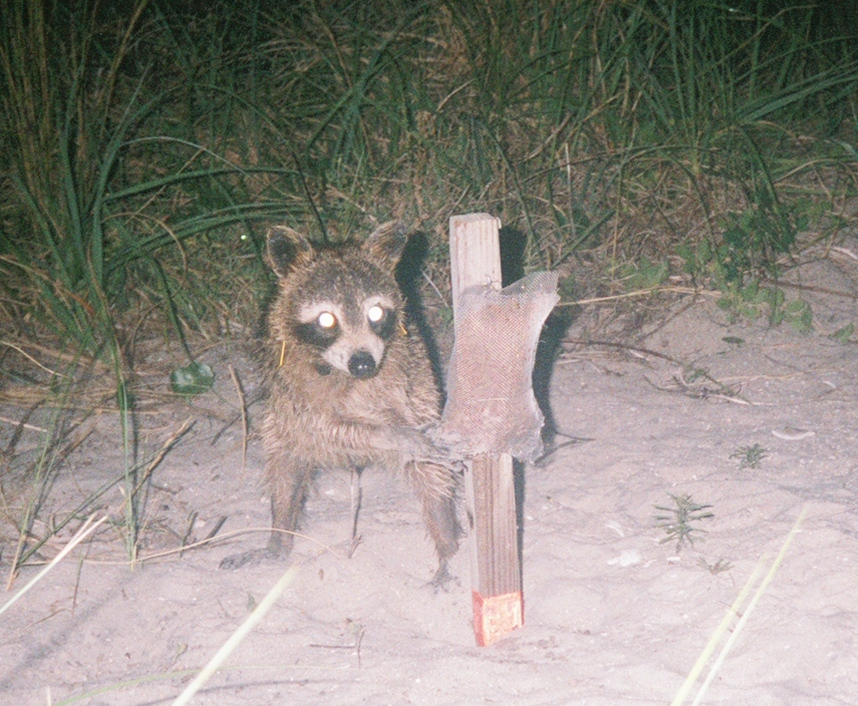
\includegraphics[width=4in]{Ch19-PartialID/figs/Raccoon_pic.png}
  \caption{Camera trap picture of a raccoon marked with a cattle tag that cannot be read to determine individual identity. Taken on South Core Banks, North Carolina.
({\it Photo credit: Arielle Parsons})}
  \label{partialID.fig.raccoon}
\end{figure}

The state-space ${\cal S}$ was the entire area of South Core Banks island. A change in the number of photocaptures over the course of the study suggested a variation of detection rate with time. Since date recording in cameras malfunctioned, photographic records could only be assigned to the time interval between subsequent trap checks, and these intervals between checks are referred to as sampling occasions. These occasions ranged from 2 to 43 days; $\lambda_0$ was standardized to 7-day intervals and allowed to change with sampling occasion. Since not all pictures of marked raccoons could be identified to the individual level, the authors applied the correction factor $c$ as described in sec. \ref{partialID.sec.IDrate}, estimated separately for each occasion.

Camera-traps recorded 117 pictures of unmarked raccoons, 33 pictures of 18 marked and identifiable raccoons, and 49 records of marked but not individually identifiable individuals (Fig. \ref{partialID.fig.raccoon}). An average of 16.32 telemetry locations (SD 4.91) were collected for each of the 38 collared individuals. Raccoon abundance on the island was estimated at 186.71 (SE 14.81) individuals, which translated to a density of 8.29 (SE 0.66) individuals per $km^2$. Parameter estimates are listed in Tab. \ref{partialID.tab.raccoons}.

\begin{table}%[hb]
\centering
\caption{Summary statistics of posterior distributions 
from spatial mark-resigh model for raccoon camera trapping and telemetry data. Baseline trap encounter rate $\lambda_0$ was standardized to 7-day intervals; $\lambda_0$ and the probability of identifying a picture of a marked individual, $c$, were allowed to vary among the 6 sampling occasions (t); $\sigma$ is estimated from telemetry data of 38 radio-collared individuals.}
\begin{tabular}{lrrrrr}
\hline
   &	Mean (SE) &	2.5\% &	50\%	& 97.5\% \\
 \hline
$N$	& 186.71 (14.81) & 162 & 185	& 220 \\
$D$	& 8.29 (0.66)	& 7.19	& 8.22	& 9.77 \\
$\lambda_0$ (t=1)	& 0.24 (0.05) & 0.16 & 0.23 & 0.34 \\
$\lambda_0$ (t=2)	& 0.40 (0.08)	& 0.26	& 0.39	& 0.57 \\
$\lambda_0$ (t=3)	& 0.11 (0.03) & 0.06 & 0.11	& 0.17 \\
$\lambda_0$ (t=4)	& 0.30 (0.07)	& 0.17	& 0.29	& 0.46 \\
$\lambda_0$ (t=5)	& 0.03 (0.01)	& 0.02	& 0.03	& 0.06 \\
$\lambda_0$ (t=6)	& 0.03 (0.01)	& 0.02	& 0.03	& 0.05 \\
$\sigma$	& 0.49 (0.01)	& 0.47	& 0.49	& 0.51 \\
$c$ (t=1)	& 0.55 (0.09)	& 0.38	& 0.55	& 0.71 \\
$c$ (t=2)	& 0.39 (0.11)	& 0.18	& 0.39	& 0.62 \\
$c$ (t=3)	& 0.29 (0.11) & 0.11	& 0.29	& 0.52 \\
$c$ (t=4)	& 0.38 (0.16)	& 0.10	& 0.36	& 0.71 \\
$c$ (t=5)	& 0.38 (0.16)	& 0.10	& 0.36	& 0.71 \\
$c$ (t=6)	& 0.30 (0.14)	& 0.08	& 0.29	& 0.60 \\
 \hline
\end{tabular}
\label{partialID.tab.raccoons}
\end{table}

In this study, although a large number of raccoons were tagged, photographic data of these tagged individuals were surprisingly sparse. Analysis of the photographic data set without the telemetry data did not render usable estimates as parallel Markov chains did not converge. One reason for the relatively sparse data was the camera trap study design: traps were spaced on average 1.77 km apart, which is about 3.5 times $\sigma$. Consequently, very few individual raccoons were photographed at more than one trap. Under these circumstances, the telemetry data provide the necessary spatial information to estimate $\sigma$ and the activity centers of individual animals and thus make other model parameter estimable. Similarly, in a camera-trapping study on Florida panthers (\emph{Puma concolor coryi}), \citet{sollmann_etal:inprepjapplecol}, including telemetry data from the 3 individuals that were collared and known to use the study area resulted in density estimates with considerably higher precision as compared to preliminary estimates \emph{without} telemetry location data, reducing the width of the 95 \% BCI by about 60 \%. Such improvements in precision of estimates is especially important when we are interested in changes in the population over time.

\section{Marked animals are not a random sample from the state-space}
XXX I dont like this heading but cannot think of anything else XXXXX
As discussed in sec. \ref{partialID.sec.random}, all the previously developed SMR models assume that marked individuals are a random sample, both spatially and demographically, from the population of the state-space. For many studies it may not be feasibly to strive to meet or approximate this assumption and it is thus important to generalize SMR models to situations where marking did not take place throughout {\cal S}. If you think about it, even if you set up marking traps throughout the state-space, individuals at the border of {\cal S} would be exposed to fewer traps and be less likely to be caught, thus creating a gradient in the proportion of marked to unmarked animals (although if {\cal S} is large enough this is probably negligible). Here, we will consider two approaches to dealing with this situation: (1) where individuals are a random (uniformly distributed) sample from a smaller region within {\cal S}, say {\cal B}; and (2) where we assume that the distribution of marked individuals follows a bivariate normal distribution around the centriod of an array of marking locations (or, generally, an area over which animals were marked), $Xm_c$. 

\subsection{Marked animals are uniformly distributed in a smaller area}
Imagine we perform an area search in a square, {\cal B}, for some species we want to study, maybe a reptile, and we mark all individuals we encounter. We conduct our sampling in a way that we can assume that the individuals we marked are uniformly distributed in {\cal B}. This also entails the assumption that {\cal B} can be clearly defined. We will come back to these assumptions in a minute. We then perform resighting surveys of some sort in an area that overlaps {\cal B}, so that, when we set a state-space around our resighting locations, {\cal B} is completely contained within {\cal S}, and we assume that the number of marked animals, $m$, is known. We further assume that individuals that were marked in {\cal B} continue to live within {\cal B} when resighting surveys are conducted, i.e. their activity centers do not shift during the complete mark-resight study. That means that we assume population closure across both the marking and the resighting part of the study. 

Let the total population of {\cal B} be $N_B$.
Under the conditions specified above, the number of marked animals $m$ can be described as the outcome of a binomial random variable
\[
m \sim {\mbox Binomial}(\theta, N_B)
\]  
where $\theta$ is the probability that an animal living in {\cal B} is marked. Remember that, by definition, all marked animals live inside {\cal B}. We now have to make sure that unmarked individuals get distributed across {\cal S} and {\cal B} so that {\emph overall} density is constant. 
Let {\cal A} be ${\cal S} - {\cal B}$, i.e., the area of {\cal S} {\emph not} covered by {\cal B}. Then, the proportion of $N$ that should fall inside {\cal B}, say $\pi_B$, can be expressed as ${\cal B}/({\cal A}+{\cal B})$. Consequently, the proportion of $N$ in {\cal A}, $\pi_A$, is ${\cal A}/({\cal A}+{\cal B})$. 
Conditioning these proportions on being an unmarked animal, we obtain
\[
pi_B|unmarked = (1-\theta)*pi_B
pi_A|unmarked = 1 - pi_B|unmarked
\]
And we can use these conditional probabilities as prior probabilities for the activity centers of unmarked individuals. 
In other words, we now have two sets of priors for activity centers. For marked animals, $[s_i]\sim \mbox{Uniform}({\cal B})$. For unmarked animals, we introduce a binary variable, say $b$, and let $b=1$ mean that $s_i$ lies within {\cal B}; then $[s_i]\sim \mbox{Bernoulli}(pi_B|unmarked)$.  
Because manipulating areas that are not simple rectangles (in this example, {\cal A}) in {\bf JAGS} is not straight forward, we wrote our own MCMC algorithm for this model, which can be found in the {\tt scrbook} package by invoking {\tt scrPIDBox}. A full example of how to simulate and analyze data under this model is given on the help page for {\tt scrPIDBox}.  

The above described model is an approach to specifying a spatial reference frame for marked individuals if these are not sampled uniformly from {\cal S}, and provides us with the ability to distribute unmarked individuals proportionally between the marking area and the rest of the state-space, so that an overall uniform density is obtained. Some of the assumptions of the model, however, are reminiscent of traditional capture-recapture and thus, suffer from the same shortcomings. {\cal B} needs to be clearly defined as the area the marked individuals live in, but how do we define it? Imagine again that {\cal B} is a quadrad search plot. Surely, we could capture an individual at the edge of the plot, whose activity center is located {\emph off} that plot. Not accounting for this effect, we will overestimate density in {\cal B}. This is the equivalent of  having to define an effective area sampled in traditional capture-recapture in order to estimate density. Further, we assume that $\theta$, the probability of an individual within the plot being marked is the same for all individuals in {\cal B}. But we discussed early on in this book that this is unlikely to be true, because exposure to sampling depends on an individual's home range overlap with the sampled area. So individuals near the edge of {\cal B} are less likely to be marked than those in the center, assuming we dispense marking effort uniformly across {\cal B} (maybe we could counteract this effect to some extent by creating a decreasing gradient of sampling effort from the edge of the plot to the center).  

We can look at this approach from a slightly different angle. Effectively, what we do here is combine a non-spatial capture recapture model -- more specifically, model $M_0$ with equal capture probability -- for the marking process with a spatial mark-resight model for the resighting process. In our simplified example, we only have a single marking occasion, but we can estimate $\theta$, the probability of being captured and marked, because we have enough information about how many unmarked individuals occur in {\cal B} coming from the spatial resighting model. While the underlying assumptions of the non-spatial marking model are questionable, we believe that the idea of combining marking and resighting into a unified model holds the key to developing a generalized spatial mark-resight model that does not rely on animals being marked throughout {\cal S}, at least when marking and resighting occur in a short enough time frame that the population can be assumed closed. As such, in spite of some shortcomings, the present approach is an important conceptual step forward. Including the marking process provides a spatial context for marked individuals, so that the resighting part of the model is no longer sensitive to the choice of the state-space. The next step will be to develop a fully spatial mode, where both the marking and the resighting process are spatially explicit.      

XXX prob be good to make a figure here XXXXX
\subsection{Marked animals follow a bivariate normal distribution around the centroid of the marking array}
In this approach we assume that marking of animals takes place across some area, and that marking effort is distributed uniformly throughout this area, e.g, if we have an array of traps, there is no ``hole'' in the array. 


\section{Summary and Outlook}
In this chapter we combined SCR models and the spatial model for unmarked populations to derive a spatial mark-resight model, which accomodates that part of the population is individually identifiable, usually through artificial tags. The basic model with known number of marked individuals and 100 \% individual identification of marked is easily modified for situations where the number of marked individuals is unknown, or where marked animals can sometimes not be identified to individual level. As expected, having marked individuals in the study population improved accuracy and precision of parameter estimates when compared to fully unmarked populations, but we also saw that the spatial counts of unmarked individuals still contribute information to parameter estimates. Finally, we present an approach of how to incorporate telemetry location data into the spatial mark-resight model to inform estimates of $\sigma$ and activity centers. Especially for difficult-to-study, cryptic species where often only a small sample of the population can be tagged this enables researchers to make optimal use of all existing data and obtain robust density estimates without the need for additional invasive methods. Just as SCR, the spatial mark-resight model framework is flexible to account for a variety of factors that may influence individual movement and detection, as well as survey-related parameters, and we saw one example for the Canada geese, where $\sigma$ was sex-sepcific.

Spatial mark-resight models are a fairly new development and much remains to be explored. We mentioned the assignment of marked but unidentified records to actual marked individuals based on their spatial location, which provides some (though imperfect) information of their identity (sec. \ref{partialID.sec.IDrate}). Similarly, records where the marked status cannot be determined could potentially be included in the model as some form of overall correction factor on detection. GPS telemetry devices and their ability to collect location data with much higher frequency offer the opportunity to assign records of collared animals to individuals based on how close to a given camera the collared individuals were, both in space and time. In this scenario, individual identity itself could be expressed probabilistically, leading to an SMR model accouting for potential misidentification. All these possible extensions can tailor SMR models to specific survey techniques. As such, the approach is applicable to a wide range of population estimation problems when dealing with animals that cannot be identified based on natural marks.


% \subsection{Sensitivity to the state-space}

% While the formulation of spatial mark-resight models for a known
% number of marked indivduals, $m$, is straight forward, these model
% have one major caveat: because we fix the size of the marked part of
% our population, total population size $N$ no longer scales with the
% area of the state-space. While the number of unmarked individuals can
% go up as ${\cal S}$ increases in size, $m$ is fixed by design. If our
% data contain all-zero encounter histories for some of the marked
% individuals, we have no immediate information about where in the
% state-space these never observed individuals live (apart from the
% vague information that they probably do not live in the middle of the
% trap array). As we increase ${\cal S}$, the area over which these marked
% unobserved individuals can live increases, too -- and consequently,
% their density decreases.  As a result, we find that density estimates
% from spatial mark-resight models with a known number of marks are
% sensitive to choice of the state-space -- as we increase ${\cal S}$,
% density estimates go down.  This is, of course, a highly undesirable
% quality in a density model. {\bf XXXXX Not a property of the model,
%   but rather of misspecifying something! We need to figure this
%   out.... XXXXXX}
% While this is an area of active research,
% we believe that under certain circumstances, the problem of
% sensitivity to the state-space can be avoided: If all marked animals
% are resighted at least once, we have some information about where in
% the state-space they live -- their activity centers must be close
% enough to the trap array for them to be resighted on it. Thus, even if
% we increase the overall state-space, the possible locations for the
% activity centers of the marked individuals remain limited. The effect
% is that, irrespective of the state-space, the marked individuals refer
% to a constant area, instead of getting `diluted'. Even if marked
% individuals are not resighted, we might have other sources of
% information on where they resided during our study, such as telemetry
% locations. Again, this information gives us the ability to fix the
% area the marked individuals refer to irrespective of the size of ${\cal
%   S}$, avoiding bias in density estimates. For an example of how to
% include telemetry data into spatial mark-resight models, see
% Sec. \ref{partialID.sec.telemetry}. A third option that we have not
% formally explored ourselves is to explicitly include capture locations
% of marked individuals into the model. Once again, this would provide
% some spatial reference for the location of marked individuals within
% the state-space. Lastly, there are circumstances under which we know
% the exact state-space in which individuals were marked and are being
% resighted. For example, if we study the population of some species on
% an island, and the entire island's population is potentially exposed
% to marking efforts (see the raccoon example in
% Sec. \ref{partialID.sec.telemetry}). In this case there is no
% arbitrariness in choosing ${\cal S}$ -- it is the island. If none of
% these avenues is an option, there is always the possibility of
% treating the number of marked individuals as unknown (see
% Sec. \ref{partialID.sec.unknown}), which might be more realistic under
% most field situations anyway. You should not that while we discussed
% the problem of underestimating density with an increase in
% state-space, there is also the opposite risk: if we choose ${\cal S}$
% too small so that it does not contain the activity centers of all of
% the marked individuals, but we assume, by fixing $m$, that they are
% all part of the population, we will overestimate density -- just as we
% would if we chose ${\cal S}$ too small in a regular SCR setting. All
% this just emphaizes what we already stated in Chapt. \ref{chapt.scr0}:
% the state-space is an integral part of your spatial capture-recapture
% (or mark-resight) model and some thought should go into specifying it
% adequately.

% \subsection{MCMC for a spatial mark-resight model}

% Implementing a spatial mark-resight model in {\bf JAGS} is not
% trivial, % XXXX See the "scratch" directory and the .jag files for
%          % some examples of working around this issue in JAGS
% since the program does not accept partially observed
% multivariate nodes (in this case the partially observed individual
% encounter histories which we model as coming from a multinomial
% distribution). Therefore, knowing how to write your own MCMC algorithm
% comes
% in 
% handy. You will find that we only have to make relatively
% simple modifications to the MCMC code we developed for regular SCR models in
% Chapt. \ref{chapt.mcmc}.
% Essentially, since we observe individual detections for the marked part of the population, we have to update only the unobserved part of ${\bf Y}$, and
% modify the updating steps for $z_i$ and $\psi$, the parameters introduced by data augmentation, to reflect some
% contribution to our
% knowledge of these parameters from the $m$ marked individuals.

% First, we set up an array to hold ${\bf Y}$, fill the first $m$ rows
% of the array with the $m$ observed individual encounter histories,
% then update ${\bf Y}$ for the unknown individuals only (note that the
% code is set up so that $n_{jk}$ contains both pictures of marked {\bf
%   and} unmarked individuals at $j$ and $k$):


% {\small
% \begin{verbatim}
% # set up placeholders and create vectors for marked and unmarked
%  Y <- array(NA, c(M, J, K))
%     nMarked <- nrow(y)
%     marked <- rep(FALSE, M)
%         marked[1:nMarked] <- TRUE
%         Y[1:nMarked, , ] <- y
%     z[marked] <- 1
%     Ydata <- !is.na(Y)
%     for (j in 1:J) {
%         for (k in 1:K) {
%             if (y[j, k] == 0) {
%                 Y[, j, k] <- 0
%                 next
%             }
%             unmarked <- !Ydata[, j, k]
%             nUnknown <- n[j, k] - sum(Y[!unmarked, j,k])
%             if (nUnknown < 0)
%                 browser()
%             probs <- lam[, j] * z
%             probs <- probs[unmarked]
%             probs <- probs/sum(probs)
%             Y[unmarked, j, k] <- rmultinom(1, nUnknown, probs)
%         }
%     }
% \end{verbatim}
% }

% When we know the number of marked individuals in the population estimating $N$ is reduced to etimating $U$. Thus, we only need to estimate the $z_i$ for $M-m$ unknown individuals and the updater for $z_i$ becomes:
% {\small
% \begin{verbatim}
% zUps <- 0
% seen <- apply(Y > 0, 1, any)
%    for (i in 1:M) {
%        if (seen[i] | marked[i])
%                 next
%        zcand <- ifelse(z[i] == 0, 1, 0)
%        ll <- sum(dpois(Y[i, , ], lam[i, ] * z[i], log = TRUE))
%        llcand <- sum(dpois(Y[i, , ], lam[i, ] * zcand,
%                   log = TRUE))
%        prior <- dbinom(z[i], 1, psi, log = TRUE)
%        prior.cand <- dbinom(zcand, 1, psi, log = TRUE)
%           if (runif(1) < exp((llcand + prior.cand) - (ll +
%                 prior))) {
%           z[i] <- zcand
%           zUps <- zUps + 1
%             }
%         }
% \end{verbatim}
% }
% Observe that while we skip the update of $z_i$ for the ``seen'' individuals (where  {\tt seen=TRUE} for any individual observed at least once and {\tt seen=FALSE} otherwise), {\tt seen} is defined based on ${\bf Y}$ and ${\bf Y}$ is updated at each iteration, so the $z_i$ for the observed but unmarked individuals are still updated.

% Finally, our update for $\psi$ needs to reflect that we are effectively only estimating $U$. In the full conditional beta distribution we have to replace $M$ with $M-m$ and $\sum z$ with $\sum z -m$:
% {\small
% \begin{verbatim}
%   psi<-rbeta(1,1+sum(w[!marked]),1+sum(!marked)-sum(w[!marked]))
% \end{verbatim}
% }
% The remainder of the code is essentially identical to the MCMC code for regular SCR models we developed in Chapt. \ref{chapt.mcmc}.
% You can find the full MCMC code (including the modeling options we'll discuss in the following sections) in the accompanying {\bf R} package {\tt scrbook} by invoking {\tt scrPID}.

% \subsection{Binomial encounter model}
% So far, we have only worked with Poisson encounter models for
% partially identifiable or unmarked populations. When we use a
% Bernoulli model instead, we have to make some changes to how we update
% the latent $y_{ijk}$, to ensure that a hypothetical individual
% receives at most a single observation at a given trap and occasion
% from the pool of $n_{jk}$ pictures. Thus, we move from a multinomial
% model
% where the same individual could be drawn repeatedly, to a sampling
% without replacement model(an individual drawn once at $j$ and $k$
% cannot be drawn again). The resuting full conditional distribution of
% the latent encounter histories is called a multivariate hypergemetric
% distibution; here is how we implement this in our MCMC algorithm:

% {\small
% \begin{verbatim}
%  Y <- array(NA, c(M, J, K))
% #[...]
%     for (j in 1:J) {
%         for (k in 1:K) {
%             if (y[j, k] == 0) {
%                 Y[, j, k] <- 0
%                 next
%             }
%             unmarked <- !Ydata[, j, k]
%             nUnknown <- n[j, k] - sum(Y[!unmarked, j,k])
%             if (nUnknown < 0)
%                 browser()
%             probs <- lam[, j] * z
%             probs <- probs[unmarked]
%             probs <- probs/sum(probs)
%             Y[unmarked, j, k] <- 0
%             guys <- sample(which(unmarked), nUnknown, prob = probs)
%             Y[guys, j, k] <- 1
%         }
%     }
% \end{verbatim}
% }


% {\bf R} makes it easy to implement the update of $\sigma$ and ${\bf
%   s}_i$ based on telemetry data and the above described full
% conditionals within our existing MCMC algorithm. We replace the
% current updating step for $\sigma$ with:
% {\small
% \begin{verbatim}
% #ntot = number of telemetry-tagged individuals
% #locs = list of length ntot; each element is a matrix
% #with telemetry locations
% #telID = vector with identifier for telemetry-tagged
% #individuals

% sigma.cand <- rnorm(1, sigma, delta[1])
% if (sigma.cand > 0) {

% llsig<-llsig.cand<-rep(NA, ntot)

% for (x in 1:ntot) {
% lls[x]<-sum(dmvnorm(x=locs[[x]],mean=c(S[telID[x],1],S[telID[x],2]),
% 			sigma=cbind(c(sigma^2,0), c(0,sigma^2)), log=T))
% lls.cand[x]<-sum(dmvnorm(x=locs[[x]],mean=c(S[telID[x],1],S[telID[x],2]),
% 	sigma=cbind(c(sigma.cand^2,0), c(0,sigma.cand^2)), log=T))
% 	}
%    if(runif(1) < exp( sum(lls.cand)  - sum(lls) ) ){
%     sigma<-sigma.cand
%     lam <- lam0*exp(-(D*D)/(2*sigma.cand*sigma.cand))
% 					}
% 			}
% \end{verbatim}
% }
% For the ${\bf s}_i$ we use an analogous updater for the
% telemetry-tagged individuals and the regular updater for individuals
% without associated telemetry location information. 
% A full example can
% be found in the {\bf R} package {\tt scrbook}, by calling {\tt
%   scrPID.tel}. 

